\chapter{Lesson 6}
\section{Overview}
In lesson one of this special feature on learning the guitar, we were introduced to the parts of the guitar, learned to tune the instrument, learned a chromatic scale, and learned Gmajor, Cmajor, and Dmajor chords. Guitar lesson two taught us to play Eminor, Aminor, and Dminor chords, an E phrygian scale, a few basic strumming patterns, and the names of the open strings. In guitar lesson three, we learned how to play a blues scale, Emajor, Amajor, and Fmajor chords, and a new strumming pattern. Lesson four introduced us to power chords, basic note names on the sixth and fifth string, and new strumming patterns. Most recently, in lesson five, we studied sharps and flats, were introduced to barre chords, learned to read tab, and learned a basic 12 bar blues. If you are not familiar with any of these concepts, it is advised that you revisit these lessons before proceeding.

\subsection{What You'll Learn in Lesson Six}
Hopefully, you won't find this lesson so tough. We'll tackle a few new chords, which are called 7th chords. Also, we'll learn a few more of the tricky barre chords. Plus, a new handy strumming pattern. Additionally, if you looking for warm-up exercises, we'll learn a movable chromatic scale pattern. And, as usual, we'll get down to applying what we've learned, by using these techniques in various songs. 

Are you ready? Good, let's start guitar lesson six.

\section{Chromatic Scale}
If you think all the way back to lesson one, you'll recall we previously learned a chromatic scale pattern. We used that scale as a means of getting our fingers accustomed to pressing down frets on the guitar. Here again, we will study another method of playing this scale, except farther up on the neck. The goal of learning this new scale position is to get our fretting hand to move smoothly and quickly all over the neck.

Before we begin, let's clarify exactly what a "chromatic scale" is. In Western music, there are 12 different musical pitches (A, Bb, B, C, Db, D, Eb, E, F, Gb, G, Ab). The chromatic scale includes EACH of these 12 pitches. So, we could actually play a chromatic scale simply by sliding our finger up one string, playing each fret.

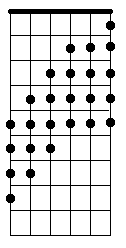
\includegraphics{partsix/chromaticscale2octave.png}

Our reason for learning the chromatic scale, at this point, is simply as a means of improving our finger technique. Start by placing your first finger on the fifth fret of the sixth string, and play that note with a downstroke. Follow that by using your second finger to play the sixth fret of the sixth string (with an upstroke). Then, your third finger should play the seventh fret on the sixth string, and lastly, your fourth (pinky) finger should play the eighth fret.

Now, move on to the fifth string. Playing this string will require a "position shift" in your fretting hand. Move your hand position down one fret, starting on the fourth fret of the fifth string with your first finger. Play each note on that string, as you did on the sixth. Repeat this process on each of the sixth strings (notice that you DON'T switch positions on the second string. This is because the second string is tuned differently than the other five.)

When you reach the first string, play the first fret with your first finger, as usual. Then, immediately switch positions, and also play the second fret with your first finger. This step allows you to reach the fifth fret, thus completing the two octave A chromatic scale. When you've reached the end of the scale, try playing it backwards.

\subsection{Remember}
\begin{itemize}
\item Keep your fretting hand as loose as possible. Don't grip the neck too tightly, or switching positions will become more difficult.
\item Try and set up a steady rhythm while playing the scale. Focus on making it sound as fluid as possible. Play the scale as slowly as necessary in order to make the tempo even throughout.
\item Alternate picking here is extremely important. Don't allow yourself to be careless.
\item Try looking at your picking hand while you play, instead of at your fretting hand. Is it doing everything as efficiently as it should?
\item Don't rush through this exercise, and don't allow yourself to get frustrated. Pay careful attention to any minor flaws in your technique, and try to remedy them.
\end{itemize}
Let's move on to learning the 7th chords... 

\section{Open 7th Chords}
Up until this point, we've dealt with only major, minor, and 5th(power) chords. While these are all extremely common, there are many other types of chords, each of which have their own unique sound. The 7th chord (aka the 7 chord) is one of these many different chords. This week, we'll look at a few of these 7th chords, in open position (not barre chords).

\subsection{Playing a G7 chord}
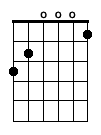
\includegraphics{partsix/openg7.png}

Start playing the G7 chord by placing your third finger on the third fret of the sixth string. Next, put your second finger on the second fret of the fifth string. Lastly, place your first finger on the first fret of the first string. Make sure your fingers are nicely curled, and give the chord a strum. Voila! Notice that this G7 chord looks quite similar to a Gmajor chord - only one note is different.

\subsection{Playing a C7 chord}
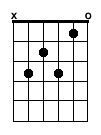
\includegraphics{partsix/openc7.png}

The C7 chord shouldn't give you too much trouble - it again is very close in formation to a Cmajor chord, with only one note being different. Play this chord as follows - form a Cmajor chord, by placing your third finger on the third fret of the fifth string, your second finger on the second fret of the fourth string, and your first finger on the first fret of the second string. Now, place your fourth (pinky) finger on the third fret of the third string. Strum the bottom five strings, and you're playing a C7 chord.

\subsection{Playing a D7 chord}
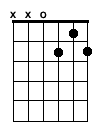
\includegraphics{partsix/opend7.png}

As with the previous two chords, you'll notice the D7 chord is rather similar to the Dmajor chord. Start by placing your second finger on the second fret of the third string. Next, place your first finger on the first fret of the second string. Lastly, put your third finger on the second fret of the first string. Strum the bottom four strings, and you're playing a D7 chord.

\subsection{Remember}
\begin{itemize}
\item In all cases, you should be checking each chord for accuracy by playing strings one at a time. If each string does not ring clearly, find out why not, and correct the problem.
\item Be sure you're not strumming strings with an "x" above them in the diagrams. Playing these strings will almost always result in chords sounding yucky.
\item Practice moving from chord to chord, saying each one aloud as you're playing it. It is very important to memorize the chord name as well as the chord shape.
\end{itemize}
Let's move on to learning more barre chords.

\section{Barre Chord Basics}
In lesson five, we took the big step of beginning to play barre chords, by learning a B minor chord. If you haven't practiced B minor recently, I'd suggest taking some time to try and master it before continuing. Knowing the note names on the sixth and fifth strings is also required to properly use barre chords.

The barre chords in lesson six will be somewhat similar to the shape we learned previously. These chords are difficult to play at first, but with practice, they will begin to open up whole new worlds in your guitar playing. 

\subsection{The F major barre shape}
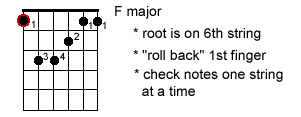
\includegraphics{partsix/fmajorbarre.png}

As with the Bminor chord, the key to playing this F major shape well is getting your first finger to flatten across the entire fretboard. Try rolling your first finger back slightly, towards the headstock of the guitar. Once your first finger feels firmly in place, try adding your other fingers to complete the chord. Playing this shape well requires much practice, but it WILL get easier, and soon you won't understand why these shapes ever caused you any problems.

As with the Bminor chord in our last lesson, this major chord shape is a "movable chord". Meaning, we can slide this chord up and down the neck, in order to play different major chords. The root of the chord is on the sixth string, so whatever note you are holding down on the sixth string is the letter name of that major chord. For example, if you were playing the chord at the fifth fret, it would be an A major chord. If you were playing the chord at the second fret, it would be a Gb major chord (aka F\# major). 

\subsection{The F minor barre shape}
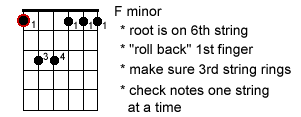
\includegraphics{partsix/fminorbarre.png}

This chord is very similar to the Fmajor shape above. There is only one slight difference... your second finger is not used at all. Your first finger is now responsible for fretting four of the six notes in the chord. Although it looks slightly easier to play than the major chord, many guitarists initially have a harder time making the chord sound correct. When playing the chord, pay careful attention to the third string. Is the note ringing clearly? If not, try and correct the problem. Playing these chords well will take time - don't allow yourself to get frustrated! It took me months to get them to sound as clearly as I liked. Try to keep that in mind.

Again, this minor chord is a movable shape. If you played this chord on the 8th fret, you'd be playing a C minor chord. On the 4th fret, you'd be playing an Ab minor chord (aka G\# minor). 

\subsection{Using Barre Chords}
Once you get the hang of playing these new shapes, you can start to use them everywhere. One of the best ways to practice barre chords is to try using them in songs you already know how to play. Simply use barre chords instead of the open chords you were using previously. Try playing Leaving on a Jet Plane using the major barre chord shapes, for example. 

\subsection{Things to Try}
\begin{itemize}
\item If you're feeling overwhelmed, try playing any songs you know that use an F major chord. Play all other chords in the song with "regular" open chord shapes, but try the barre shape for the F major.
\item Make a sincere effort to learn note names on the sixth and fifth string. I can't stress enough how important this is to learn.
\item Play barre chords for just a few minutes every day - but play them EVERY DAY. You'll be surprised how quickly you learn them. 
\end{itemize}
Now, let's move on to a new strumming pattern. 

\section{Strumming Patterns}
In lesson two, we learned all about the basics of strumming the guitar. We added another new strum to our repetoire in lesson three. In lesson four, we studied yet another common strumming pattern. If you still aren't comfortable with the concept and execution of basic guitar strumming, it is advised that you return to those lessons and review. 

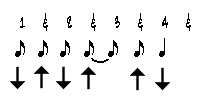
\includegraphics{partsix/strum5.png}

If you didn't have any problems with prior strumming patterns, then this one won't give much difficulty either. This is another common strum, which is just a slight variation of several strums covered earlier.

Let's take a moment to listen to what this strumming pattern sounds like at a slow tempo. Try and internalize the rhythm of this strum before you even attempt to play it on guitar. Say "down up down up up down" along with the audio clip. Once you feel comfortable that you know the rhythm properly, pick up your guitar, hold down a G major chord, and try strumming along.

If you can't seem to get it right, spend more time practicing the rhythm away from your guitar. I can't stress this enough - the key to learning strumming patterns is to be able to "hear" the pattern in your head before you try and play it. Once you've gotten the hang of it, you'll want to try playing the same pattern at a faster tempo 

\subsection{Remember}
\begin{itemize}
\item If you are playing an acoustic guitar, make sure to strum directly over the sound hole
\item On electric guitar, strum over the body (different locations will give you different sounds), not over the neck
\item Make sure all strings are ringing clearly
\item Make sure the volume of your downstrums and upstrums are equal
\item Be careful not to strum too hard, as this often causes strings to rattle, and produces an undesirable sound
\item Be careful not to strum too softly, as this will produce a "wimpy" sound. Your pick should be striking the strings with a relatively firm, even stroke
\item Think of your elbow as being the top of a pendulum; your arm should swing up and down from it in a steady motion, never pausing at any time.
\item Having said that, the bulk of the picking motion should come from a rotation of the wrist, rather than from the forearm. Be sure not to keep your wrist stiff when playing. 
\end{itemize}
Let's use these new chords and strumming patterns by learning some new songs. 

\section{Learning Songs}
Since we've now covered all the basic open chords, plus power chords, and now the B minor chord, there are a countless number of songs to tackle. This week's songs will be focus on both open and power chords. 

Best of my Love - performed by The Eagles
NOTES: We can use our newest strum to play this song, which also includes a G7 chord we learned this week. The bridge includes an Fminor barre chord, but if you can't play that yet, at least attempt the verse.
Californication - performed by The Red Hot Chili Peppers
NOTES: This is the title track from the band's 2000 album. Some single notes to learn, but the song isn't too hard.
Hotel California - performed by The Eagles
NOTES: we did this one last lesson as well, but you'll be better equipped to play it now. Try using full barre chords for Bminor and F\#major. When you see Bm7, play Bminor. Strum: down down up up down up
Yer So Bad - performed by Tom Petty
NOTES: if you're getting frustrated, here's a nice, easy song to learn. Just a few chords, none of them new. For now, we'll strum it down down up up down up.

\section{Practice Schedule}
Don't spend all of your time trying to play barre chords - chances are you'll just end up frustrated with very sore fingers. If you want to conquer them, however, you'll have to put in a few minutes worth of work every time you pick up your guitar. Here are some other things you'll want to practice after this lesson:
\begin{itemize}
\item First, make sure your guitar is in tune).
\item Warm up by playing the new chromatic scale slowly and accurately. Try not to hesitate when switching strings.
\item Review the new 7th chords, plus open chords, power chords, the B minor barre chord, and this week's barre chords. We've learned a lot, so it's important to keep them all organized in your mind.
\item Review all strumming patterns we've covered. We've learned patterns in lesson two, lesson three, lesson four, and lesson six. Try switching from chord to chord while using these patterns.
\item Try to play all of the songs above, plus keep playing those from previous lessons. Try committing one or several songs to memory. Pick an easy one to start with. 
\end{itemize}
As we continue to learn more and more material, it becomes easy to overlook the techniques we learned during earlier lessons. They are all still important, so it is advisable to keep going over older lessons, and be sure you're not forgetting anything. There is a strong human tendency to only practice things which we are already quite good at. You'll need to overcome this, and force yourself to practice the things you are weakest at doing.

If you're feeling confident with everything we've learned so far, I suggest trying to find a few songs you're interested in, and learn them on your own. You can use the easy guitar tab area of the site to hunt down the music that you'd enjoy learning the most. Try memorizing some of these songs, rather than always looking at the music to play them.

In lesson seven, we'll another barre chord (our last for a little while), hammer-on and pull-off techniques, new songs, and much more. Be sure you're always having fun while you're playing, and keep smiling! 

